\lstdefinelanguage{plaintext}{
  sensitive=false,
  comment=[l]{//},
  morecomment=[s]{/*}{*/},
  identifierstyle=\color{black},
  morestring=[b]',
  morestring=[b]"
}

\lstset
{ 
    language=plaintext,
    basicstyle=\footnotesize,
    numbers=left,
    stepnumber=1,
    showstringspaces=false,
    tabsize=1,
    breaklines=true,
    breakatwhitespace=false,
    frame=leftline
}

\chapter{Perancangan}
\label{chap:Perancangan}

Pada bab ini dibahas mengenai perancangan perangkat lunak yang dibangun, meliputi perancangan kelas dan algoritma pengecekan dokumen skripsi.

\section{Perancangan Kelas}
Pada bagian ini akan dijelaskan rancangan kelas yang akan digunakan pada perangkat lunak. Rancangan kelas tersebut akan ditunjukan oleh diagram kelas di bawah ini:

\begin{figure}[H]
	\centering	
	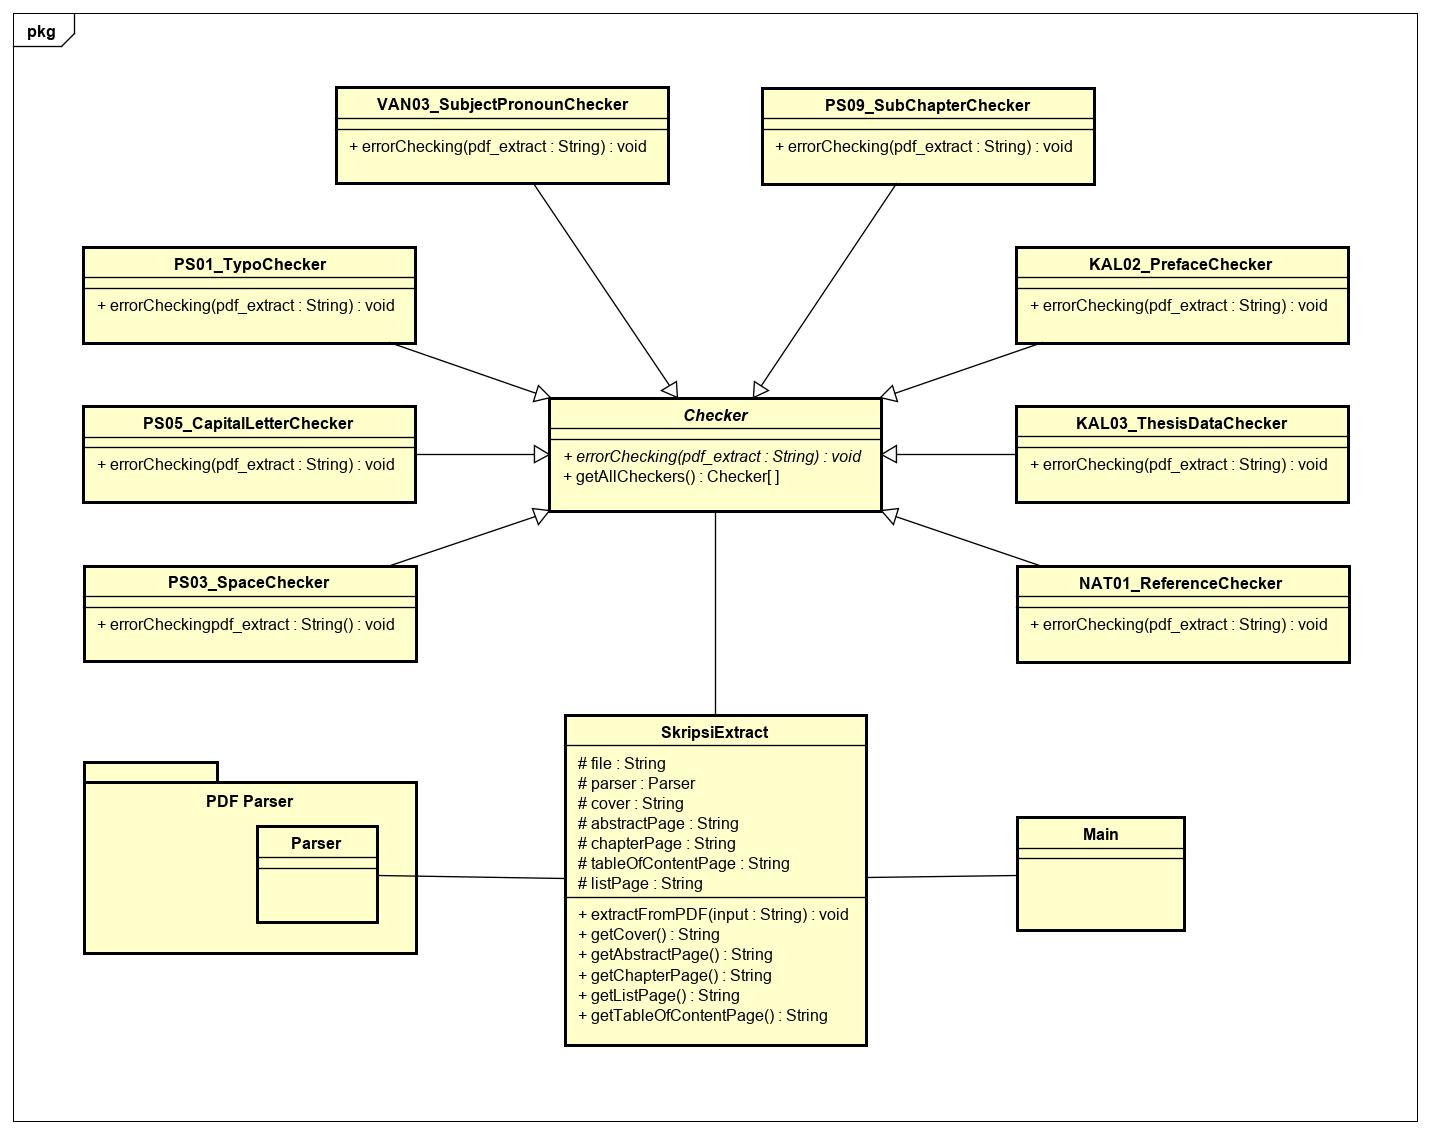
\includegraphics[scale=0.44]{class-diagram.png}
	\caption{Diagram kelas Aplikasi Pemeriksa Kesalahan Dokumen Skripsi}	
	\label{fig:diagram_kelas} 
\end{figure}

Pada gambar \ref{fig:diagram_kelas} telah ditunjukan bahwa perangkat lunak memiliki sebelas kelas dan sebuah \textit{library PDF Parser}. Rincian dari setiap kelas tersebut akan dijelaskan sebagai berikut:

\begin{enumerate}

	\item Kelas Checker \\
	Kelas ini merupakan kelas \textit{Parent} dari semua \textit{checker} yang akan diimplementasi pada perangkat lunak. Berikut adalah \textit{method} yang terdapat pada kelas ini:
	
		\begin{itemize}
			\item errorChecking(\$pdf\_extract) \\
			Method ini merupakan method abstrak, yang akan diturunkan kepada seluruh anak kelasnya. Method ini berfungsi untuk memeriksa kesalahan pada dokumen skripsi sesuai dengan peran yang diberikan pada kelas tersebut. Method ini menerima masukan pdf\_extract dengan tipe data kelas \textit{SkripsiExtract}. Parameter tersebut dapat digunakan oleh masing-masing kelas \textit{Checker} untuk memanggil \textit{method getter} yang diperlukan. Tidak semua pemeriksa memerlukan seluruh isi halaman dari dokumen skripsi.			
			
			\item getAllChecker() \\
			Method ini berfungsi untuk melakukan instansiasi seluruh anak kelas \textit{Checker}. Method ini mengembalikan hasil instansiasi anak kelas \textit{Checker}.
		\end{itemize}
	
	\item Kelas KAL02\_PrefaceChecker \\
	Kelas ini bertanggungjawab untuk memeriksa ada atau tidaknya kata pengantar sebelum memulai bab atau subbab. Berikut adalah \textit{method} yang terdapat pada kelas ini:
	
		\begin{itemize}
			\item errorChecking(\$pdf\_extract) \\
			Method ini berfungsi untuk memeriksa kesalahan pada dokumen skripsi. Method ini menerima masukan pdf\_extract dengan tipe data kelas \textit{SkripsiExtract}. Bagian yang diperiksa pada \textit{checker} ini hanya bab 1 hingga 6.
		\end{itemize}
	
	\item Kelas KAL03\_ThesisDataChecker \\
	Kelas ini bertanggungjawab untuk memeriksa kelengkapan data skripsi yang ditulis dalam bahasa Indonesia maupun bahasa Inggris. Berikut adalah \textit{method} yang terdapat pada kelas ini:
			
		\begin{itemize}
			\item errorChecking(\$pdf\_extract) \\
			Method ini berfungsi untuk memeriksa kesalahan pada dokumen skripsi. Method ini menerima masukan pdf\_extract dengan tipe data kelas \textit{SkripsiExtract}. Bagian yang diperiksa pada \textit{checker} ini adalah halaman cover bahasa Indonesia dan bahasa Inggris.
		\end{itemize}
		
	\item Kelas NAT01\_ReferenceChecker \\
	Kelas ini bertanggungjawab untuk memeriksa referensi yang akan dirujuk dalam dokumen. Berikut adalah \textit{method} yang terdapat pada kelas ini:
	
		\begin{itemize}
			\item errorChecking(\$pdf\_extract) \\
			Method ini berfungsi untuk memeriksa kesalahan pada dokumen skripsi. Method ini menerima masukan pdf\_extract dengan tipe data kelas \textit{SkripsiExtract}. Bagian yang diperiksa pada \textit{checker} ini adalah bab 1 hingga 6.
		\end{itemize}
			
	\item Kelas PS01\_TypoChecker \\
	Kelas ini bertanggungjawab untuk memeriksa kesalahan penulisan kata. Berikut adalah \textit{method} yang terdapat pada kelas ini:
	
		\begin{itemize}
			\item errorChecking(\$pdf\_extract) \\
			\textit{Method} ini berfungsi untuk memeriksa kesalahan pada dokumen skripsi. Method ini menerima masukan pdf\_extract dengan tipe data kelas \textit{SkripsiExtract}. Bagian yang diperiksa pada \textit{checker} ini adalah bab 1 hingga 6.
		\end{itemize}
			
	\item Kelas PS03\_SpaceChecker \\
	Kelas ini bertanggungjawab untuk memeriksa penggunaan spasi sebelum dan setelah tanda baca. Berikut adalah \textit{method} yang terdapat pada kelas ini:	
	
		\begin{itemize}
			\item errorChecking(\$pdf\_extract) \\
			\textit{Method} ini berfungsi untuk memeriksa kesalahan pada dokumen skripsi. Method ini menerima masukan pdf\_extract dengan tipe data kelas \textit{SkripsiExtract}. Bagian yang diperiksa pada \textit{checker} ini adalah bab 1 hingga 6.
		\end{itemize}
			
	\item Kelas PS05\_CapitalLetterChecker \\
	Kelas ini bertanggungjawab untuk memeriksa penggunaan huruf kapital pada awal kalimat. Berikut adalah \textit{method} yang terdapat pada kelas ini:
		
		\begin{itemize}
			\item errorChecking(\$pdf\_extract) \\
			\textit{Method} ini berfungsi untuk memeriksa kesalahan pada dokumen skripsi. Method ini menerima masukan pdf\_extract dengan tipe data kelas \textit{SkripsiExtract}. Bagian yang diperiksa pada \textit{checker} ini adalah bab 1 hingga 6.
		\end{itemize}
			
	\item Kelas PS09\_SubChapterChecker \\
	Kelas ini bertanggungjawab untuk memeriksa subbab yang ada dalam sebuah bab. Berikut adalah \textit{method} yang terdapat pada kelas ini:
			
		\begin{itemize}
			\item errorChecking(\$pdf\_extract) \\
			Method ini berfungsi untuk memeriksa kesalahan pada dokumen skripsi. Method ini menerima masukan pdf\_extract dengan tipe data kelas \textit{SkripsiExtract}. Bagian yang diperiksa pada \textit{checker} ini adalah bab 1 hingga 6.
		\end{itemize}
			
	\item Kelas VAN03\_SubjectProunounChecker \\
	Kelas ini bertanggungjawab untuk memeriksa penggunaan kata ganti orang pada dokumen skripsi. Berikut adalah \textit{method} yang terdapat pada kelas ini:
	
		\begin{itemize}
			\item errorChecking(\$pdf\_extract) \\
			Method ini berfungsi untuk memeriksa kesalahan pada dokumen skripsi. Method ini menerima masukan pdf\_extract dengan tipe data kelas \textit{SkripsiExtract}. Bagian yang diperiksa pada \textit{checker} ini adalah bab 1 hingga 6.
		\end{itemize}
			
	\item Kelas SkripsiExtract \\
	Kelas ini berfungsi untuk melakukan proses ekstak dokumen PDF skripi dan disimpan menjadi beberapa bagian berdasarkan konten-konten yang pada dokumen skripsi. Kelas ini memiliki beberapa atribut yang akan dijelaskan sebagai berikut:
	
		\begin{itemize}
			\item file \\
			Atribut ini berfungsi untuk menyimpan nama file dari dokumen skripsi.
			
			\item parser \\			
			Atribut ini berfungsi sebagai instansiasi kelas Parser dari \textit{Library PDF Parser}.
			
			\item cover \\
			Atribut ini berfungsi untuk menyimpan hasil ekstrak dari halaman cover bahasa Indonesia dan bahasa Inggris.
			
			\item abstractPage \\			
			Atribut ini berfungsi untuk menyimpan hasil ekstrak dari halaman abstrak bahasa Indonesia dan bahasa Inggris.
			
			\item tableOfContentPage \\
			Atribut ini berfungsi untuk menyimpan hasil ekstrak dari halaman daftar isi.
			
			\item contentPage \\	
			Atribut ini berfungsi untuk menyimpan hasil ekstrak mulai dari bab 1 hingga bab 6.
			
			\item listPage \\
			Atribut ini berfungsi untuk menyimpan hasil ekstrak pada halaman daftar tabel, daftar gambar, daftar referensi dan lampiran.
			
		\end{itemize}
	
	Kelas ini juga memiliki \textit{method} yang berkaitan dengan proses ekstrak dokumen skripsi dan penyimpanan hasil ekstraknya. Berikut adalah \textit{method} yang terdapat pada kelas ini:
		
		\begin{itemize}
			\item extractFromPDF(\$input) \\
			Method ini berfungsi untuk melakukan proses ekstrak file PDF skripsi. Hasil dari ekstrak tersebut akan disimpan ke dalam beberapa bagian, seperti cover, halaman abstrak, dan sebagainya. 
			
			\item getCoverPage() \\
			Method ini berfungsi untuk mendapatkan halaman cover skripsi dalam bahasa Indonesia dan bahasa Inggris.
			
			\item getAbstractPage() \\
			Method ini berfungsi untuk mendapatkan halaman abstrak dalam bahasa Indonesia dan bahasa Inggris.
			
			\item getTableOfContentPage() \\
			Method ini berfungsi untuk mendapatkan halaman daftar isi.
			
			\item getListPage() \\
			Method ini berfungsi untuk mendapatkan halaman daftar isi, daftar gambar, daftar tabel dan daftar referensi.
			
			\item getContentPage() \\
			Method ini berfungsi untuk mendapatkan halaman konten skripsi dari bab 1 sampai bab 6.
			
			\item splitContentPage() \\
			Method ini memiliki fungsi yang hampir sama dengan method \textit{getContentPage}, yaitu untuk mendapatkan halaman konten skripsi. Namun, pada method ini ada beberapa proses pemisahan isi konten (per kalimat) ke dalam beberapa array. Fitur-fitur dalam perangkat lunak yang memerlukan pemeriksaan berdasarkan kalimat dapat langsung memanggil method ini. 
			
		\end{itemize}
	
	\item Kelas Main \\
	Kelas ini digunakan untuk menjalankan perangkat lunak. Kelas ini tidak memiliki atribut dan \textit{method}, hanya terdiri dari beberapa baris kode yang memanggil \textit{method} untuk mengekstrak dan memeriksa file PDF skripsi. 

\end{enumerate} 

\section{Perancangan Perangkat Lunak}
Pada bagian ini akan dijelaskan perancangan untuk mengekstrak dokumen skripsi dan pola pengecekan kesalahan yang akan digunakan pada perangkat lunak.
 
\subsection{Algoritma untuk Mengekstrak Dokumen}
Dokumen skripsi yang akan diperiksa dalam perangkat lunak merupakan file yang memiliki ekstensi \textit{PDF}. Sebelum dilakukan pemeriksaan kesalahan, dokumen tersebut perlu diekstrak terlebih dulu. Pada skripsi ini, aplikasi akan menggunakan \textit{library PDFParser} untuk mengekstrak dokumen skripsi. Pada \textit{library} tersebut, terdapat 2 metode yang dapat digunakan untuk mengekstrak dokumen.
	
\begin{lstlisting}[caption={Potongan kode untuk mengesktrak seluruh halaman dokumen}	\label{lst:all_page},language=php,xleftmargin=.2\textwidth] 
include 'vendor/autoload.php';
	
$parser = new \Smalot\PdfParser\Parser();
$pdf    = $parser->parseFile('document.pdf');
$text   = $pdf->getText();
\end{lstlisting}
	
\begin{lstlisting}[caption={Potongan kode untuk mengesktrak halaman dokumen secara spesifik}
\label{lst:specific_page},language=php,xleftmargin=.2\textwidth] 
include 'vendor/autoload.php';

$parser = new \Smalot\PdfParser\Parser();
$pdf    = $parser->parseFile('document.pdf');
$pages  = $pdf->getPages();
\end{lstlisting}
\medskip

Listing \ref{lst:all_page} dan listing \ref{lst:specific_page} merupakan potongan kode yang terdapat pada dokumentasi \textit{library PDF Parser}. Kode dari kedua listing tersebut hampir mirip, yang menjadi pembeda adalah pada baris ke-5. Listing \ref{lst:all_page} menggunakan \textit{method getText()} dan hasil dari ekstraknya disimpan menjadi sebuah kesatuan dari halaman awal hingga halaman akhir. Listing \ref{lst:specific_page} menggunakan \textit{method getPages()} dan hasil dari ekstraknya disimpan dalam sebuah array String sejumlah halaman yang ada pada dokumen.

Pada skripsi ini akan digunakan metode yang mengesktrak halaman-halaman secara spesifik. Hasil ekstrak akan disimpan dalam berdasarkan konten-konten yang ada, seperti halaman cover, abstrak, daftar isi, daftar tabel, daftar gambar dan seterusnya. Ada beberapa alasan yang mendorong untuk melakukan pemisahan konten-konten tersebut, salah satunya yaitu agar pemeriksa dapat memeriksa bagian-bagian spesifik yang dibutuhkan. Contohnya, untuk memeriksa kelengkapan data skripsi tidak perlu memeriksa seluruh isi dari dokumen, halaman yang dibutuhkan hanya cover saja. 

\subsection{Pola Pengecekan Kesalahan}
Hasil survei kesalahan-kesalahan dalam penulisan dokumen skripsi sudah disaring dan akan diimplementasikan dalam perangkat lunak. Pengecekan kesalahan tersebut akan dilakukan dengan menggunakan teknik \textit{pattern matching}. Hasil ekstrak dari PDF skripsi akan dipotong per kalimat dengan delimiter karakter titik dan spasi ke dalam sebuah array. Berikut adalah rincian dari hasil survei yang dipilih beserta penyelesaiannya:

\begin{enumerate}
	\item Penulisan kata (PS-01) \\
	Untuk mendeteksi kesalahan penulisan kata, akan digunakan ekstensi kamus bahasa Indonesia \textit{LibreOffice}. Dengan digunakan kamus tersebut, kesalahan penulisan suatu kata dapat diminimalisir. Pada skripsi ini, pemeriksaan kata-kata yang menggunakan imbuhan tidak ditangani pada masalah ini, karena keterbatasan waktu yang dimiliki. Terdapat kode yang harus diterjemahkan terlebih dahulu untuk dapat mengetahui imbuhan yang dapat digunakan dalam sebuah kata. Pola pengecekan yang digunakan akan dijelaskan pada pseudocode \ref{alg:ps01}.
		
\begin{minipage}{1.0\linewidth}
\begin{algorithm}[H]
    \caption{Typo checker function}
	\label{alg:ps01}
	\begin{algorithmic}[1]
    	\Function{ExtractFromPDF}{\$pdf\_exctract}
    		\State Input: An object from the SkripsiExtract class to call the getter method
			\State Output: An array containing error reports		
			\State $temp \gets$ Split dictionary based on newline
			\State $dictionary \gets$ Array for store dictionary
			\For{$i = 0$ to size of temp}
				\State Remove affix code from each index dictionary array 
			\EndFor
			\State $word \gets$ Call getter from class SkripsiExtract and split with non word character
			\State $typos \gets$ Array for store typos
			\For{each word in $array$}
    			\State $row \gets$ Add $index$ with 1
        		\If{$value$ not contain in $dictionary$ and $value$ not contain in $typos$}
                	\State Fill $typos$ with $value$
            	\EndIf
        	\EndFor
			\State $result \gets$ Array for store all errors report
    		\If{size of $typos$ greater than 0}
                \State Add all errors report into $result$
            \EndIf
    		\State \textbf{return} $result$
    	\EndFunction
	\end{algorithmic}
\end{algorithm}
\end{minipage}
\medskip

	Pada pseudocode \ref{alg:ps01}, pola akan memeriksa setiap kata yang ada pada indeks array. Namun untuk pemeriksaan kata ini hanya untuk kata yang menggunakan bahasa Indonesia saja. Pola akan mencocokan kata yang akan diperiksa dengan kamus bahasa Indonesia \textit{LibreOffice}. Berikut adalah contoh dari kesalahan dan laporan yang dikeluarkan:
	
	\begin{itemize}
		\item Contoh kesalahan \\
		Istilah \textit{regex} berasal dari toeri matematika dan komputer sains, yang mencerminkan sifat ekspresi dalam matematika yang disebut keteraturan.
		\item Laporan kesalahan \\
		Ditemukan penulisan kata yang tidak sesuai dengan kamus.
	\end{itemize}
	
	\item Pemberian spasi sebelum dan sesudah tanda baca (PS-03) \\
	Kesalahan ini akan terdeteksi apabila tidak ada karakter spasi sebelum ataupun sesudah tanda baca. Pola pengecekan yang digunakan akan dijelaskan pada \textit{pseudocode} \ref{alg:ps03}.
	
\begin{minipage}{1.0\linewidth}
\begin{algorithm}[H]
    \caption{Space checker function}
	\label{alg:ps03}
	\begin{algorithmic}[1]
    	\Function{ExtractFromPDF}{\$pdf\_exctract}
    		\State Input: An object from the SkripsiExtract class to call the getter method
			\State Output: An array containing error reports
			\State $result \gets$ Array for store all errors report
			\State $sentence \gets$ Call getter from class SkripsiExtract
    		\For{each sentence in $sentence$}
    			\State $row \gets$ Add $index$ with 1
				\State $pattern \gets$ Define regex /([A-Za-z0-9]*[,.!?][A-Za-z0-9])/
        		\If{$pattern$ contain in $array$}
                	\State fill $result$ with errors report
            	\EndIf
        	\EndFor
    		\State \textbf{return} $result$
    	\EndFunction
	\end{algorithmic}
\end{algorithm}
\end{minipage}
\medskip
	
	Pada pseudocode \ref{alg:ps03}, pola akan memeriksa setiap kalimat yang ada pada indeks array. Kesalahan akan terdeteksi apabila setelah tanda baca titik, koma, seru atau tanya tidak terdapat spasi yang memisahkan tanda baca dengan kata baru. Berikut adalah contoh dari kesalahan dan laporan yang dikeluarkan:
	
	\begin{itemize}
		\item Contoh kesalahan \\
		Aplikasi ini dijalankan melalui melalui terminal command Windows.laporan dari hasil kesalahan tersebut akan ditampilkan melalui terminal command Windows.
		\item Laporan kesalahan \\
		Perhatikan spasi sebelum atau setelah tanda baca.
	\end{itemize}
	
	\item Awal kalimat tidak menggunakan huruf kapital (PS-05) \\
	Kesalahan ini akan terdeteksi apabila setelah tanda baca pada akhir kalimat, karakter pertama setelah spasi menggunakan huruf kecil. Pola pengecekan yang digunakan akan dijelaskan pada \textit{pseudocode} \ref{alg:ps05}.

\begin{minipage}{1.0\linewidth}
\begin{algorithm}[H]
    \caption{Capital letter checker function}
	\label{alg:ps05}
	\begin{algorithmic}[1]
    	\Function{ExtractFromPDF}{\$pdf\_exctract}
    		\State Input: An object from the SkripsiExtract class to call the getter method
			\State Output: An array containing error reports
			\State $result \gets$ Array for store all errors report
			\State $sentence \gets$ Call getter from class SkripsiExtract
    		\For{each sentence in $sentence$}
    			\State $row \gets$ Add $index$ with 1
				\State $pattern \gets$ Define regex / $\hat{}$ ($\backslash$s[a-z][a-z0-9].*)/
        		\If{$pattern$ contain in $array$}
                	\State fill $result$ with errors report
            	\EndIf
        	\EndFor
    		\State \textbf{return} $result$
    	\EndFunction
	\end{algorithmic}
\end{algorithm}
\end{minipage}
\medskip

	Pada pseudocode \ref{alg:ps05}, pola akan memeriksa setiap kalimat yang ada pada indeks array. Kesalahan akan terdeteksi apabila karakter pertama dalam sebuah kalimat menggunakan huruf kecil. Berikut adalah contoh dari kesalahan dan laporan yang dikeluarkan:
	
	\begin{itemize}
		\item Contoh kesalahan \\ 
		aplikasi sederhana ini, dapat dimanfaatkan oleh mahasiswa Informatika Unpar secara mandiri.
		\item Laporan kesalahan \\
		Huruf pertama pada kalimat ini tidak menggunakan huruf kapital.
	\end{itemize}
	
	\item Jumlah subbab dalam 1 bab tidak boleh hanya 1 (PS-09) \\
	Kesalahan ini dapat diselesaikan dengan mencari jumlah subbab yang ada dalam sebuah bab. Pola pengecekan yang digunakan akan dijelaskan pada \textit{pseudocode} \ref{alg:ps09}.

\begin{minipage}{1.0\linewidth}
\begin{algorithm}[H]
    \caption{Subchapter checker function}
	\label{alg:ps09}
	\begin{algorithmic}[1]
    	\Function{ExtractFromPDF}{\$pdf\_exctract}
    		\State Input: An object from the SkripsiExtract class to call the getter method
			\State Output: An array containing error reports
			\State $result \gets$ Array for store all errors report
			\State $sentence \gets$ Call getter from class SkripsiExtract
    		\For{each sentence in $sentence$}
    			\State $row \gets$ Add $index$ with 1
				\State $pattern \gets$ Define regex / $\hat{}$ /
        		\If{$pattern$ contain in $array$}
                	\State fill $result$ with errors report
            	\EndIf
        	\EndFor
    		\State \textbf{return} $result$
    	\EndFunction
	\end{algorithmic}
\end{algorithm}
\end{minipage}
\medskip
	
	Pada pseudocode \ref{alg:ps09}, pola akan memeriksa setiap kalimat yang ada pada indeks array. Kesalahan akan terdeteksi apabila karakter pertama dalam sebuah kalimat menggunakan huruf kecil. Berikut adalah contoh dari kesalahan dan laporan yang dikeluarkan:
	
	\begin{itemize}
		\item Contoh kesalahan \\
		Bab 4 \newline PERANCANGAN \newline \newline 4.1 Perancangan Kelas
		\item Laporan kesalahan \\
		Pada bab ini hanya terdapat 1 subbab, lebih baik tidak perlu menggunakan subbab.
	\end{itemize}	
	
	\item Kalimat pengantar untuk setiap subbab (KAL-02) \\
	Kesalahan ini dapat dideteksi dengan melihat ada atau tidaknya kalimat setelah subbab dibuat. Pola pengecekan yang digunakan akan dijelaskan pada \textit{pseudocode} \ref{alg:kal02}.

\begin{minipage}{1.0\linewidth}
\begin{algorithm}[H]
    \caption{Preface checker function}
	\label{alg:kal02}
	\begin{algorithmic}[1]
    	\Function{ExtractFromPDF}{\$pdf\_exctract}
    		\State Input: An object from the SkripsiExtract class to call the getter method
			\State Output: An array containing error reports
			\State $result \gets$ Array for store all errors report
			\State $sentence \gets$ Call getter from class SkripsiExtract
    		\For{each sentence in $sentence$}
    			\State $row \gets$ Add $index$ with 1
				\State $pattern \gets$ Define regex / $\hat{}$ [A-Z0-9][A-Za-z] /
        		\If{$pattern$ contain in $array$}
                	\State fill $result$ with errors report
            	\EndIf
        	\EndFor
    		\State \textbf{return} $result$
    	\EndFunction
	\end{algorithmic}
\end{algorithm}
\end{minipage}
\medskip

	Pada pseudocode \ref{alg:kal02}, pola akan memeriksa setiap kalimat yang ada pada indeks array. Kesalahan akan terdeteksi apabila tidak terdapat kalimat yang mengawali bab tersebut. Berikut adalah contoh dari kesalahan dan laporan yang dikeluarkan:
	
	\begin{itemize}
		\item Contoh kesalahan \\
		Bab 4 \newline PERANCANGAN \newline \newline 4.1 Perancangan Kelas \newline 4.2 Perancangan Algoritma
		\item Laporan kesalahan \\
		Berilah kata pengantar untuk bab atau subbab.
	\end{itemize}
	
	\item Kelengkapan data skripsi (KAL-03) \\
	Kesalahan ini dapat terlihat pada halaman cover skripsi. Mahasiswa yang belum mengisi data skripsi, pada file PDFnya akan ditampilkan tulisan template pada data skripsinya.Pola pengecekan yang digunakan akan dijelaskan pada \textit{pseudocode} \ref{alg:kal03}.
	
\begin{minipage}{1.0\linewidth}
\begin{algorithm}[H]
    \caption{Thesis data checker function}
	\label{alg:kal03}
	\begin{algorithmic}[1]
    	\Function{ExtractFromPDF}{\$pdf\_exctract}
    		\State Input: An object from the SkripsiExtract class to call the getter method
			\State Output: An array containing error reports
			\State $result \gets$ Array for store all errors report
			\State $sentence \gets$ Call getter from class SkripsiExtract
    		\For{each sentence in $sentence$}
    			\State $row \gets$ Add $index$ with 1
				\State $pattern \gets$ Define regex /JUDUL BAHASA INDONESIA|JUDUL BAHASA INGGRIS|Nama Lengkap|10 digit NPM UNPAR|tahun/
        		\If{$pattern$ contain in $array$}
                	\State fill $result$ with errors report
            	\EndIf
        	\EndFor
    		\State \textbf{return} $result$
    	\EndFunction
	\end{algorithmic}
\end{algorithm}
\end{minipage}	
\medskip
	
	Pada pseudocode \ref{alg:kal03}, pola akan memeriksa halaman cover bahasa Indonesia dan bahasa Inggris. Kesalahan akan terdeteksi pada halaman cover masih terdapat kalimat yang terdapat dalam template. Berikut adalah contoh dari kesalahan dan laporan yang dikeluarkan:
	
	\begin{itemize}
		\item Contoh kesalahan \\
		<<SKRIPSI/TUGAS AKHIR>> \newline <<Judul Bahasa Indonesia>> \newline Marcell Trixie Alexander \newline <<10 digit NPM UNPAR>>
		\item Laporan kesalahan \\
		Ada data skripsi yang belum dilengkapi, data dapat diisi pada file data.tex
	\end{itemize}	
	
	\item Penggunaan kata ganti orang (VAN-03) \\
	Kesalahan ini dapat diatasi dengan memasukan kata-kata yang termasuk dalam kata ganti orang menjadi kata-kata yang tidak dapat digunakan. Pola pengecekan yang digunakan akan dijelaskan pada \textit{pseudocode} \ref{alg:van03}.

\begin{minipage}{1.0\linewidth}
\begin{algorithm}[H]
    \caption{Subject Pronoun checker function}
	\label{alg:van03}
	\begin{algorithmic}[1]
    	\Function{ExtractFromPDF}{\$pdf\_exctract}
    		\State Input: An object from the SkripsiExtract class to call the getter method
			\State Output: An array containing error reports
			\State $result \gets$ Array for store all errors report
			\State $sentence \gets$ Split PDF parsing results based on dots and space
    		\For{each sentence in $sentence$}
    			\State $row \gets$ Add $index$ with 1
				\State $pattern \gets$ Define regex /saya|kamu|dia/i
        		\If{$pattern$ contain in $array$}
                	\State fill $result$ with errors report
            	\EndIf
        	\EndFor
    		\State \textbf{return} $result$
    	\EndFunction
	\end{algorithmic}
\end{algorithm}
\end{minipage}
\medskip

	Pada pseudocode \ref{alg:van03}, pola akan memeriksa setiap kalimat yang ada pada indeks array. Kesalahan akan terdeteksi pada kalimat terdapat kata ganti orang. Berikut adalah contoh dari kesalahan dan laporan yang dikeluarkan:
	
	\begin{itemize}
		\item Contoh kesalahan \\
		Saya akan membuat aplikasi ini menggunakan bahasa pemrograman PHP.
		\item Laporan kesalahan \\
		Kalimat ini mengandung kata ganti orang.
	\end{itemize}	
	
	\item Penulisan daftar referensi (NAT-01) \\
	Kesalahan dalam penulisan daftar referensi dapat dilihat dengan munculnya tanda ''[?]'', yang menandakan bahwa referensi tersebut tidak dirujuk dengan baik. Pola pengecekan yang digunakan akan dijelaskan pada \textit{pseudocode} \ref{alg:nat01}.

\begin{minipage}{1.0\linewidth}
\begin{algorithm}[H]
    \caption{Reference checker function}
	\label{alg:nat01}
	\begin{algorithmic}[1]
    	\Function{ExtractFromPDF}{\$pdf\_exctract}
    		\State Input: An object from the SkripsiExtract class to call the getter method
			\State Output: An array containing error reports
			\State $result \gets$ Array for store all errors report
			\State $sentence \gets$ Call getter from class SkripsiExtract
    		\For{each sentence in $sentence$}
    			\State $row \gets$ Add $index$ with 1
				\State $pattern \gets$ Define regex /[?]/
        		\If{$pattern$ contain in $array$}
                	\State fill $result$ with errors report
            	\EndIf
        	\EndFor
    		\State \textbf{return} $result$
    	\EndFunction
	\end{algorithmic}
\end{algorithm}
\end{minipage}
\medskip

	Pada pseudocode \ref{alg:nat01}, pola akan memeriksa setiap kalimat yang ada pada indeks array. Kesalahan akan terdeteksi kalimat terdapat simbol ''[?]'', yang menandakan referensi tidak dirujuk dengan baik. Berikut adalah contoh dari kesalahan dan laporan yang dikeluarkan:
	
	\begin{itemize}
		\item Contoh kesalahan \\
		\textit{Regular expression} [?] adalah jenis pola teks tertentu yang dapat digunakan pada banyak aplikasi modern dan bahasa pemrograman.
		\item Laporan kesalahan \\
		Referensi tidak dirujuk dengan baik, lakukan perintah PDFLatex->BibTex->PDFLatex->PDFLatex untuk memperbaikinya.
	\end{itemize}		
	
\end{enumerate}